
\documentclass{article}
\usepackage[utf8]{inputenc}
\usepackage{minted}
\usepackage{graphicx}
\usepackage{hyperref}
\usepackage[dvipsnames]{xcolor}
\usepackage{comment}

\title{SX1276mbedshield}
\author{cmonaton }
\date{August 2019}

\begin{document}

\maketitle

\section{Matériel}

Carte nucleo F411RE + SX1276 mbed shield

\begin{figure}[H]
  \centering
  \begin{minipage}[b]{0.4\textwidth}
    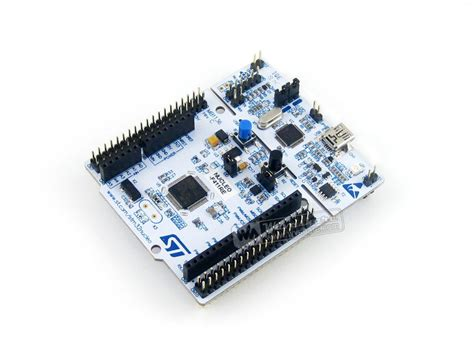
\includegraphics[width=\textwidth]{nucleo_f411re.jpeg}
    \caption{nucleo f411RE}
  \end{minipage}
  \hfill
  \begin{minipage}[b]{0.4\textwidth}
    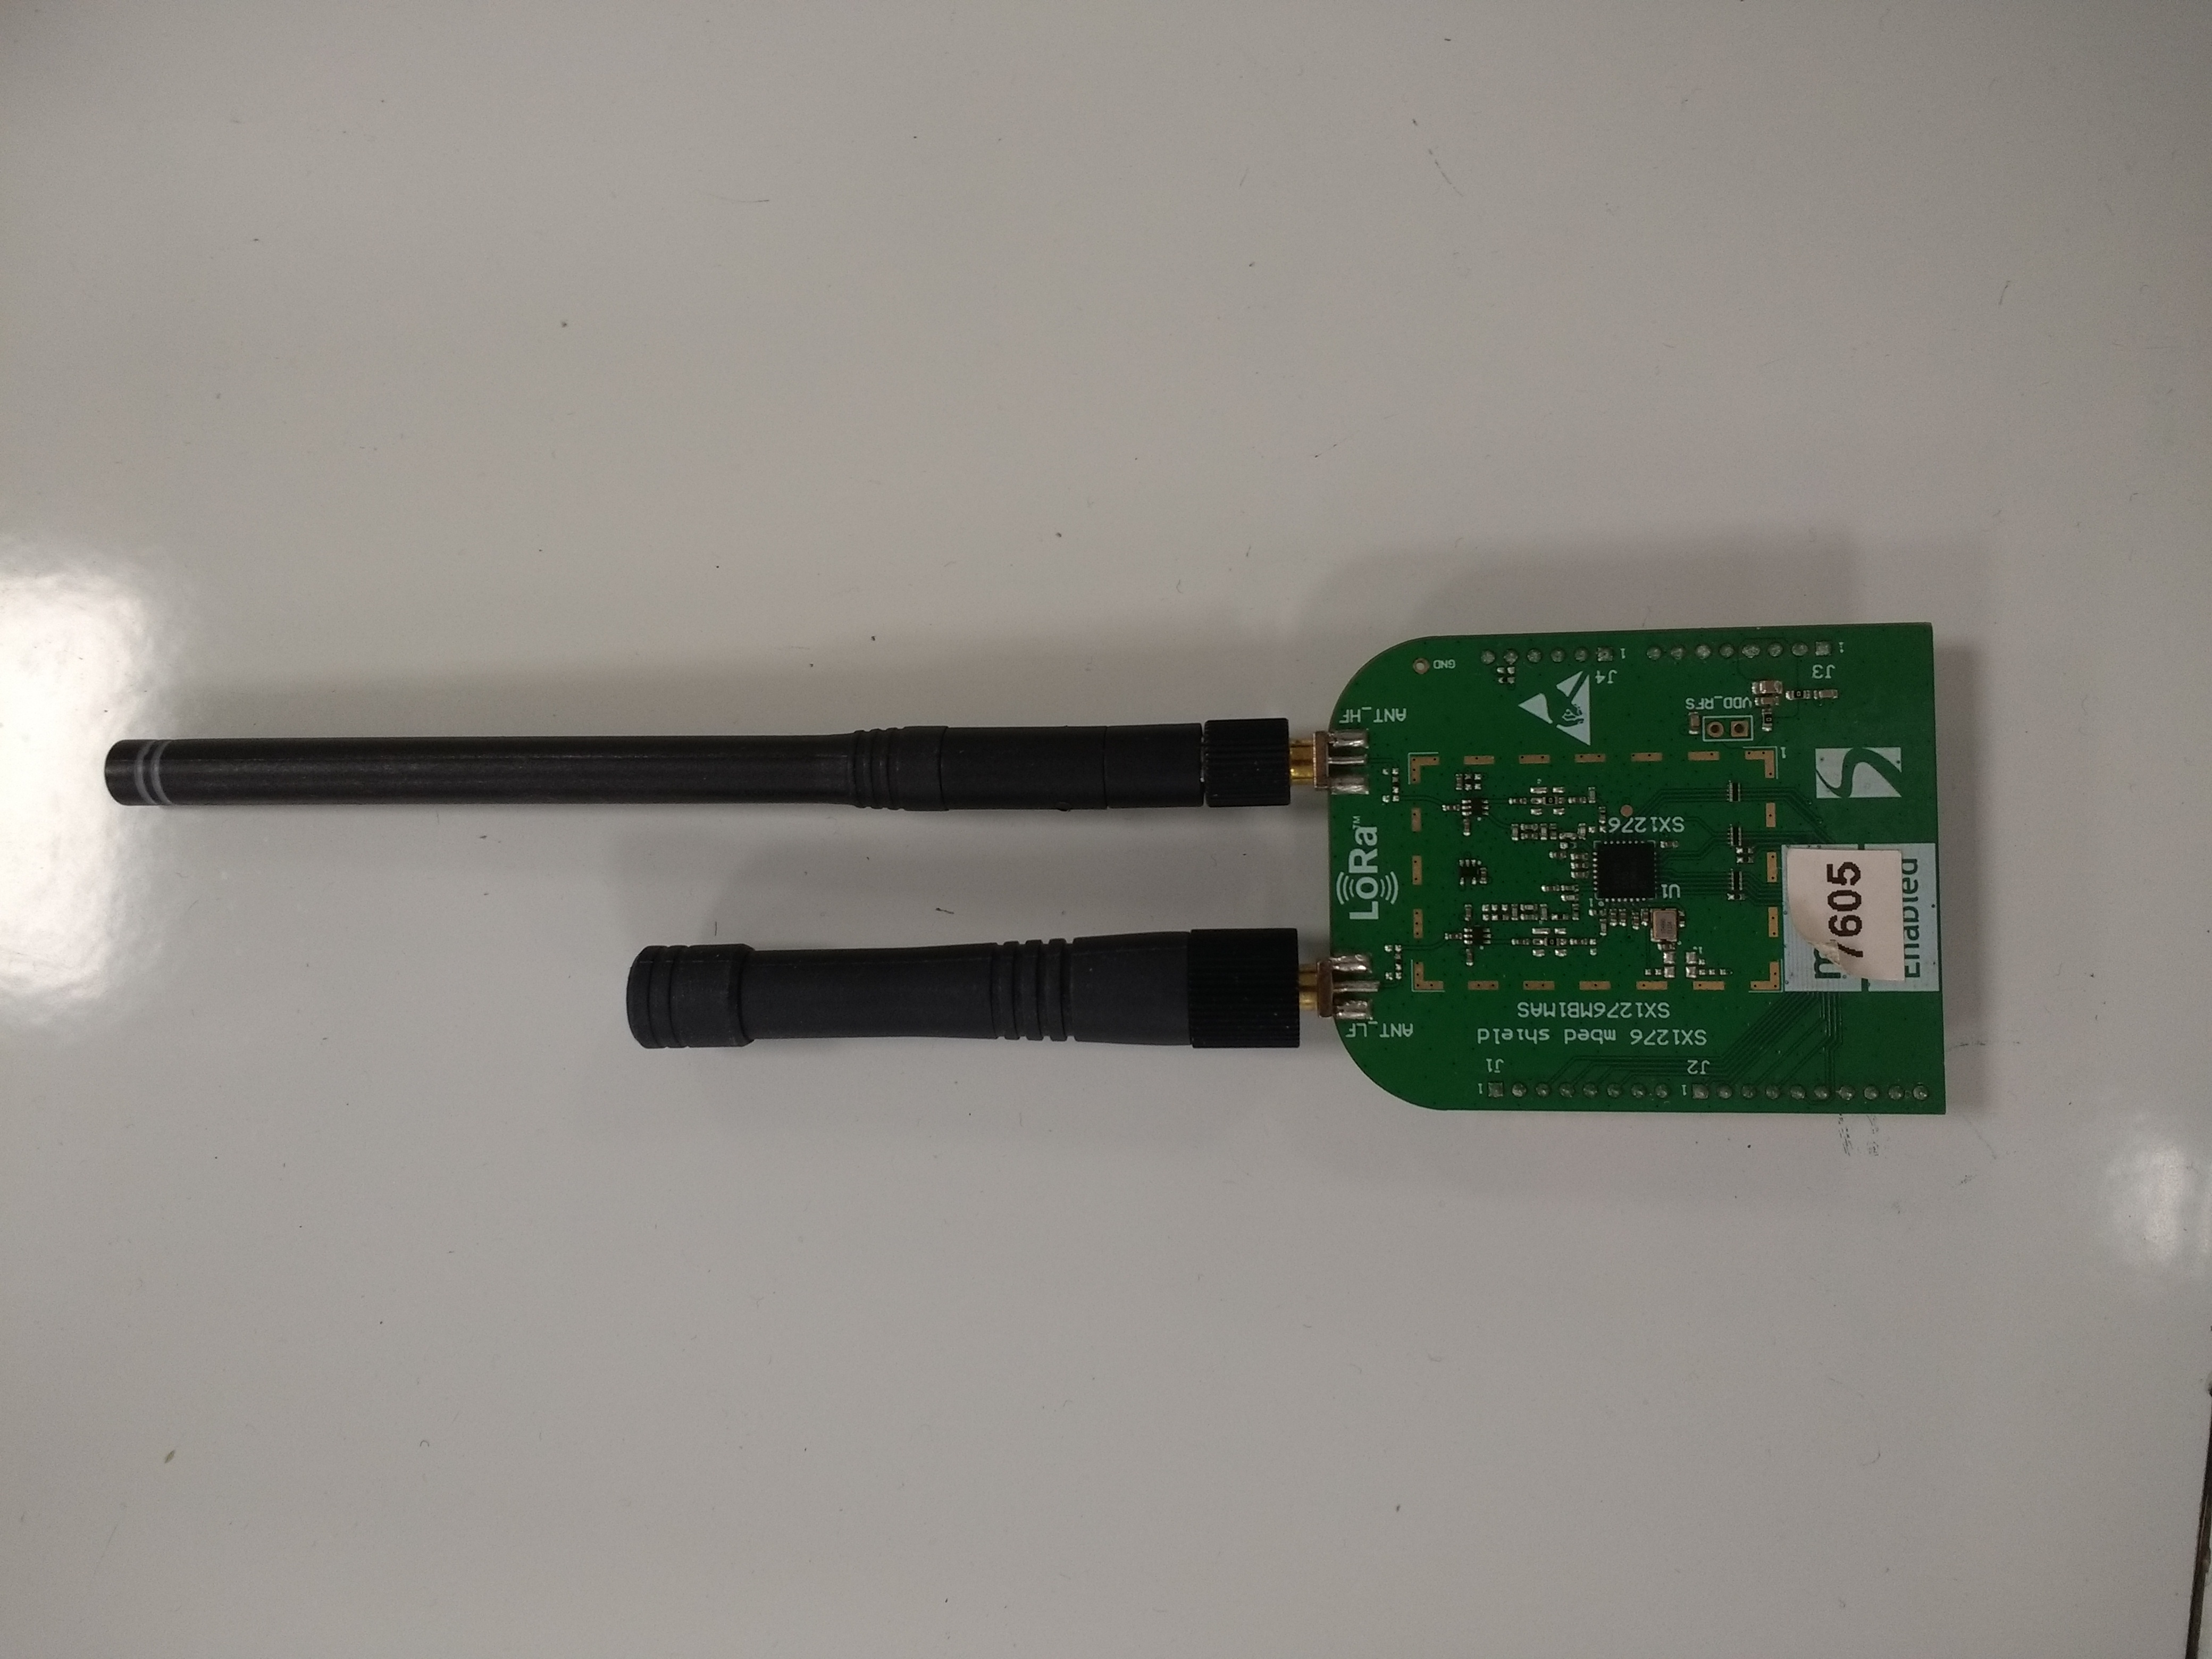
\includegraphics[width=\textwidth]{sx1276mbedshield.jpg}
    \caption{SX1276 mbed shield}
  \end{minipage}
\end{figure}


\textcolor{red}{Branchez l'antenne LoRa avant d'alimenter la carte sinon la carte grille}





\section{Générer un binaire pour la carte}

Se créer un compte sur armmbed : \url{https://www.mbed.com/en/platform/mbed-os/}

Dans l'onglet \textit{Boards}\\

\begin{figure}[H]
\begin{center}
\advance\leftskip-3cm
\advance\rightskip-3cm
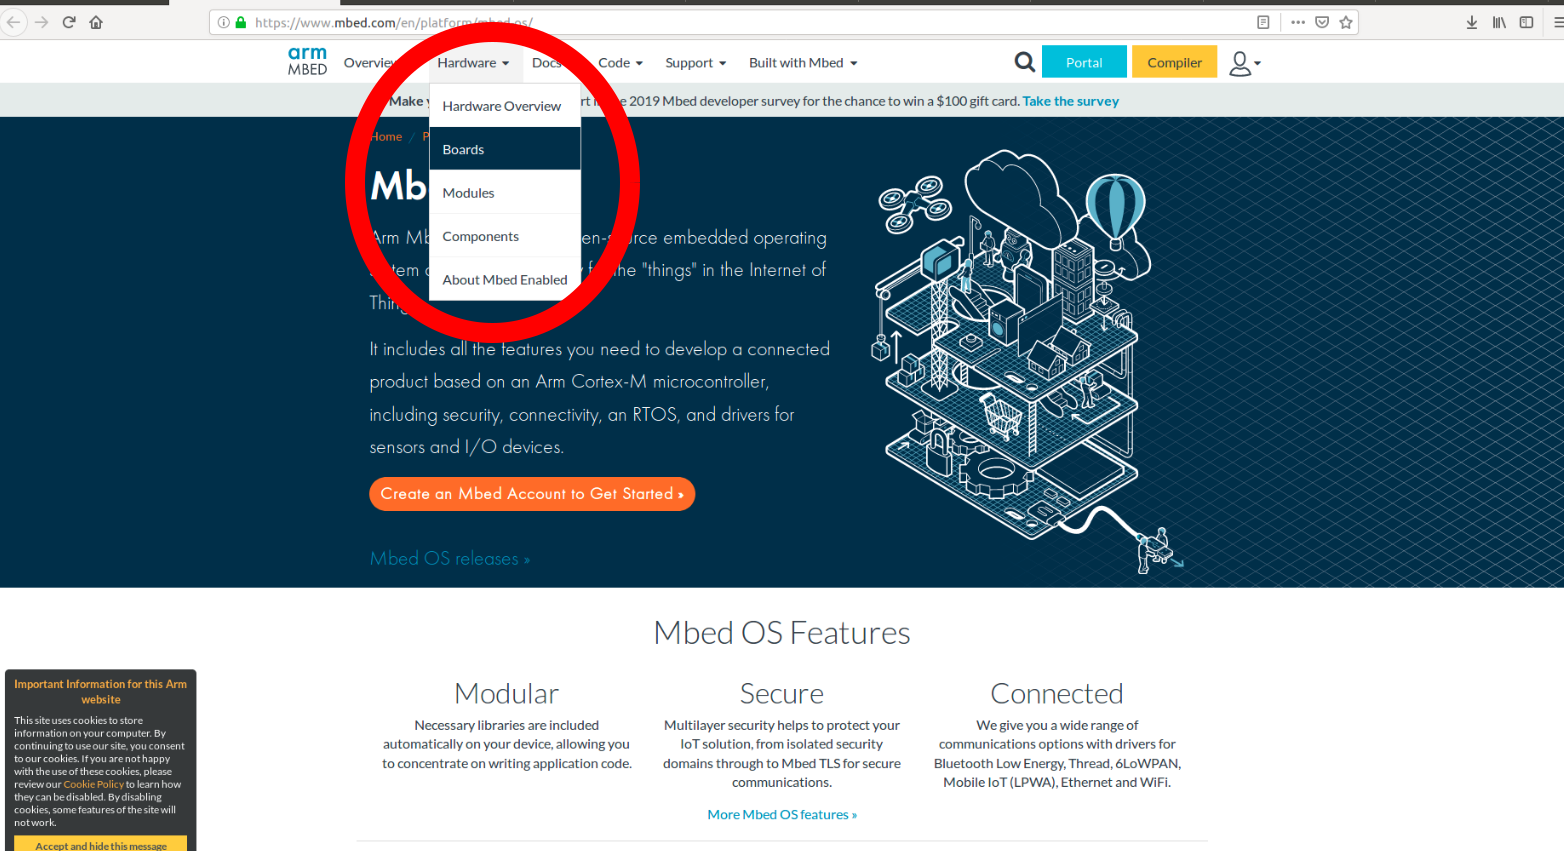
\includegraphics[keepaspectratio=true,scale=0.3]{hardawre_boards.png}
\label{visina8}
\end{center}\end{figure}

Checher la carte nucleo F411RE\\
Puis l'ajouter au compilateur : \\
\begin{figure}[H]
\begin{center}
\advance\leftskip-3cm
\advance\rightskip-3cm
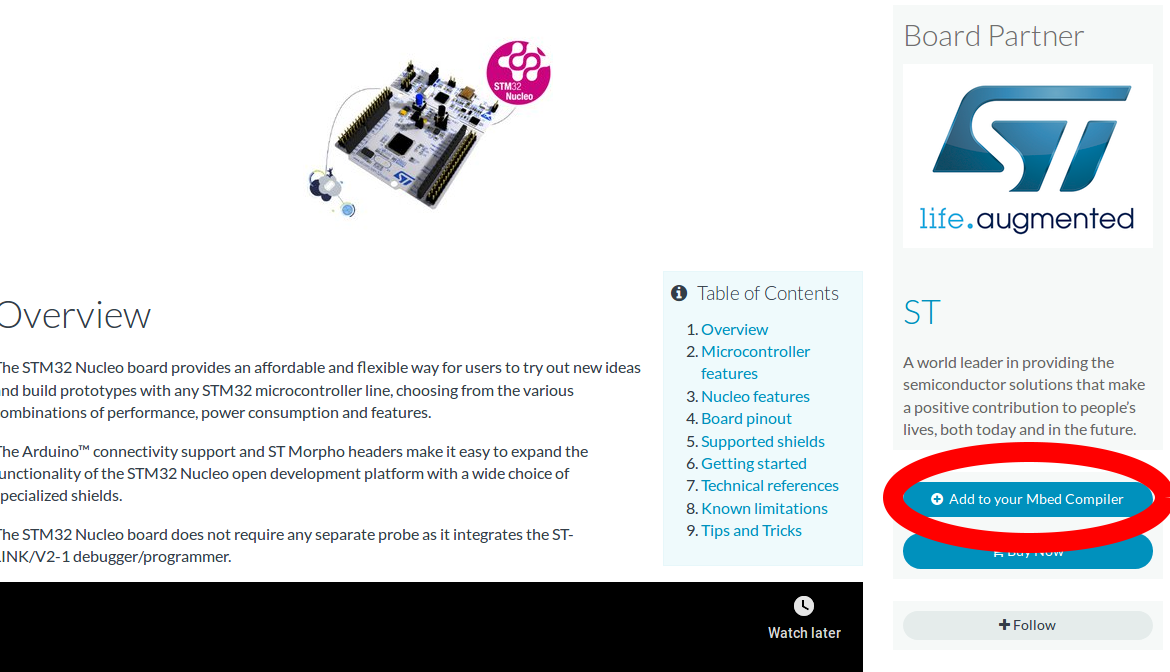
\includegraphics[keepaspectratio=true,scale=0.3]{addtocoMpiler.png}
\label{visina8}
\end{center}\end{figure}

Ouvrir le compilateur :

\begin{figure}[H]
\begin{center}
\advance\leftskip-3cm
\advance\rightskip-3cm
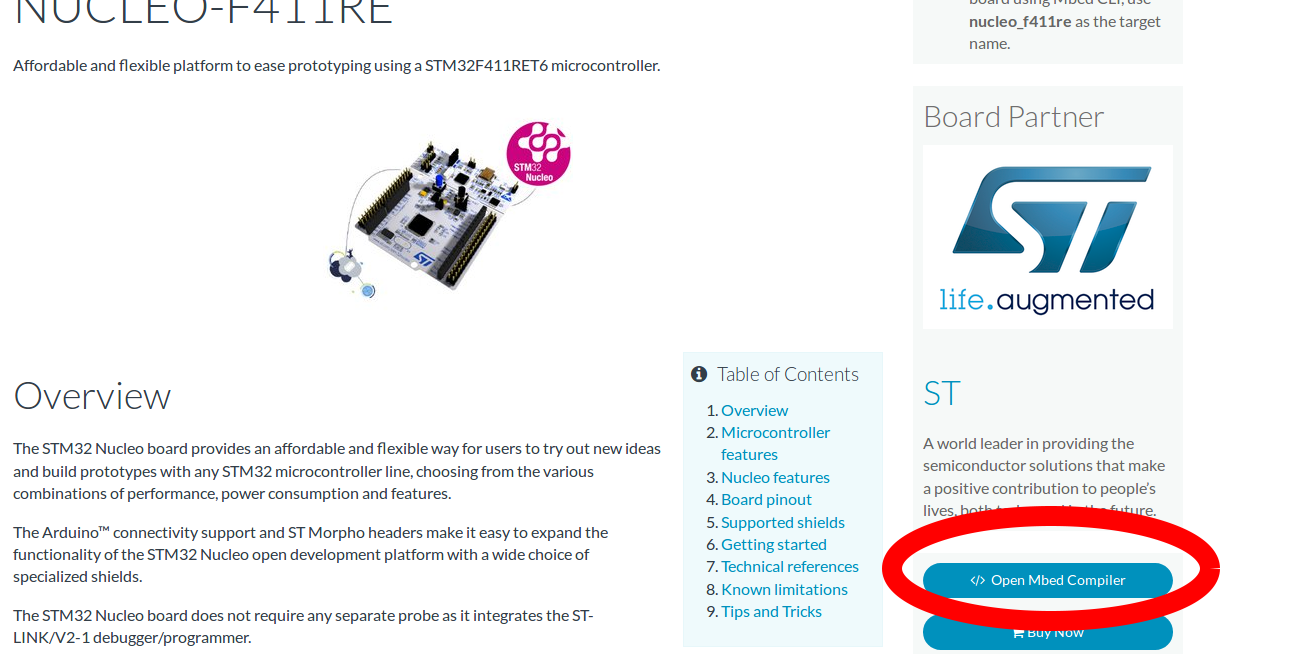
\includegraphics[keepaspectratio=true,scale=0.3]{open_mbedcompiler.png}
\label{visina8}
\end{center}\end{figure}

Choisir un programme dans la liste :

\begin{figure}[H]
\begin{center}
\advance\leftskip-3cm
\advance\rightskip-3cm
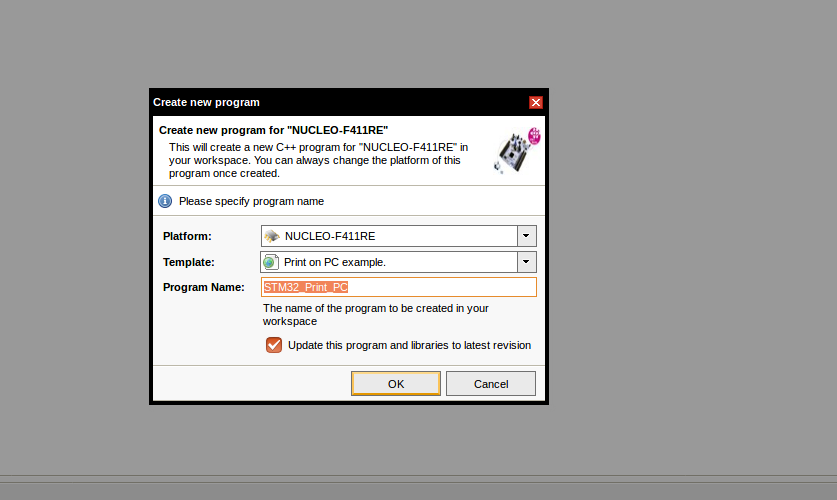
\includegraphics[keepaspectratio=true,scale=0.3]{choose_programm.png}
\label{visina8}
\end{center}\end{figure}

Compilez :
\begin{figure}[H]
\begin{center}
\advance\leftskip-3cm
\advance\rightskip-3cm
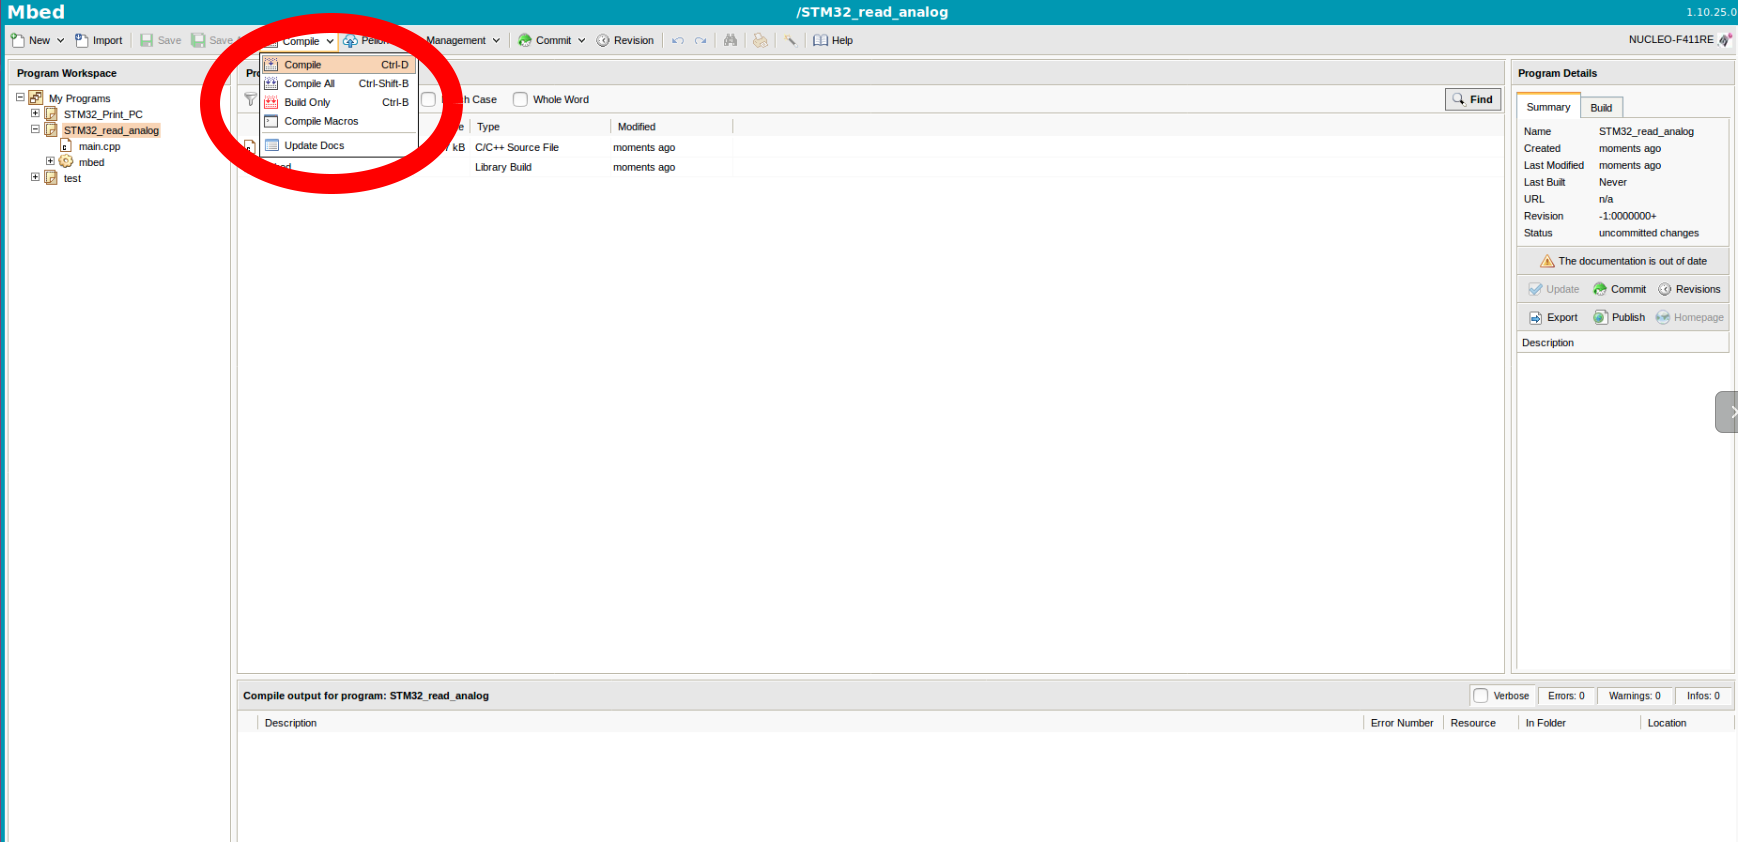
\includegraphics[keepaspectratio=true,scale=0.3]{compilE.png}
\label{visina8}
\end{center}\end{figure}

Le fichier binaire est à télécharger.

\section{Télécharger un firmware sur la carte}

Avec le logiciel STM32Cube programmer


\begin{comment}
\subsection{Installation}

\begin{itemize}
   

Sur Ubuntu 16.04.6 LTS \\

 \item Avant de lancer l'installer :
\begin{minted}{bash}

sudo apt-get install openjfx

\end{minted}

 \item Se créer un compte et télécharger le logiciel à : \\

\url{https://www.st.com/en/development-tools/stm32cubeprog.html}


Lancer l'installer .linux \\


\item  Installer libusb : \\
\begin{minted}{bash}


sudo apt-get install libusb-1.0


\end{minted}

\item Ajouter des règles dans /etc/udev/rules.d

\begin{minted}{bash}

cd /home/username/stsw-link007/AllPlatforms/StlinkRulesFilesForLinux

sudo cp *.* /etc/udev/rules.d \\
Redémarrez le PC




\end{minted}

\item Si nécessaire, upgrader STlink :

\begin{figure}[H]
\begin{center}
\advance\leftskip-3cm
\advance\rightskip-3cm
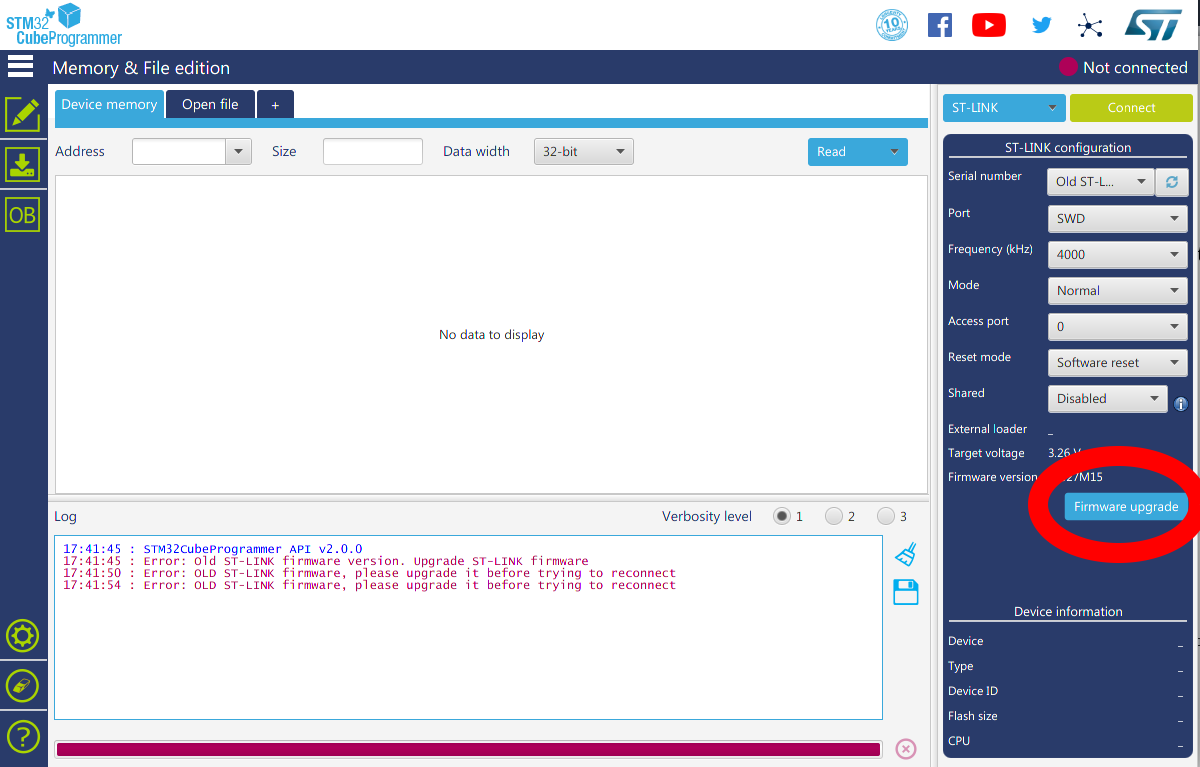
\includegraphics[keepaspectratio=true,scale=0.3]{stlink_upgrade.png}
\label{visina8}
\end{center}\end{figure}

\end{itemize}

\end{comment}

\subsection{Installation de STM32 cube programmer}
Ce logiciel permet de télécharger le code sur la carte. \\
\textit{Note}: Il semble impossible d'installer ce programme sous Ubuntu 18.04.3 LTS \\
Sur Ubuntu 16.04.6 LTS
\begin{itemize}
   
\begin{itemize}
   



 \item Avant de lancer l'installer :
\begin{minted}{bash}

sudo apt-get install openjfx

\end{minted}

 \item Se créer un compte et télécharger le logiciel à : \\

\url{https://www.st.com/en/development-tools/stm32cubeprog.html}

\begin{comment}
Lancez l'installer .linux 
\begin{minted}{bash}

./path_of_file.linux

\end{minted}
\end{comment}


\item Téléchargez STSW-LINK007 à : \\ 
\url{https://www.st.com/en/development-tools/stsw-link007.html}


\item Ajouter des règles dans /etc/udev/rules.d

\begin{minted}{bash}

cd /extraction_path/stsw-link007/AllPlatforms/StlinkRulesFilesForLinux

sudo cp *.* /etc/udev/rules.d

sudo udevadm control --reload-rules #ou rebooter le PC


\end{minted}

\end{itemize}

\subsection{Si nécessaire}

\begin{itemize}
    



\item Installer libusb

\begin{minted}{bash}


sudo apt-get install libusb-1.0


\end{minted}

\item  upgrader STlink :

\begin{figure}[H]
\begin{center}
\advance\leftskip-3cm
\advance\rightskip-3cm
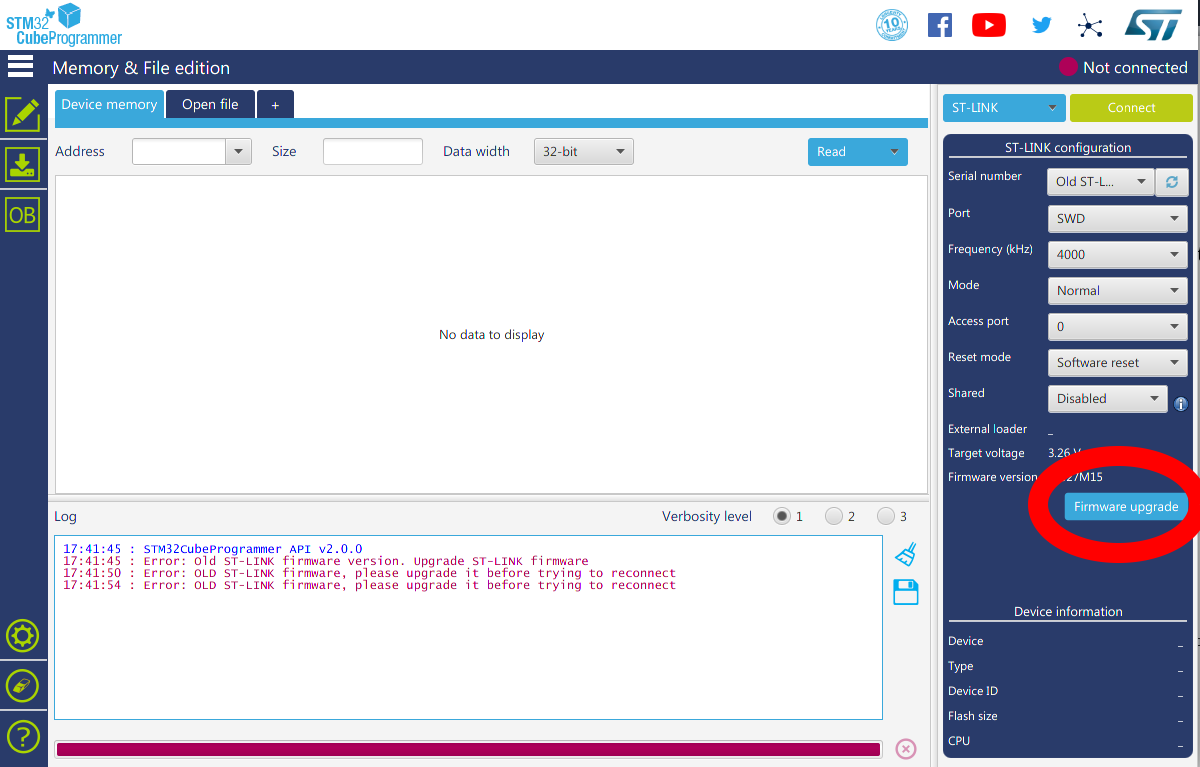
\includegraphics[keepaspectratio=true,scale=0.3]{stlink_upgrade.png}
\label{visina8}
\end{center}\end{figure}



\end{itemize}






\subsection{Téléchargement du firmware}

\begin{enumerate}


      \item Connecter la carte : Parfois la carte ne peut plus se connecter au PC pour flasher le code.
    Explication : le FW bloque le port de STLINK
    Solution : Maintenir appuyé le bouton reset de la carte au moment de la connection avec STM32Cube Programmer

    \item 
    A côté de "device memory" dans un onglet selon l'image, ajouter un fichier et "Download" un fichier .elf ou .bin \\
    
    
    
    
    
    \begin{figure}[H]
\begin{center}
\advance\leftskip-3cm
\advance\rightskip-3cm
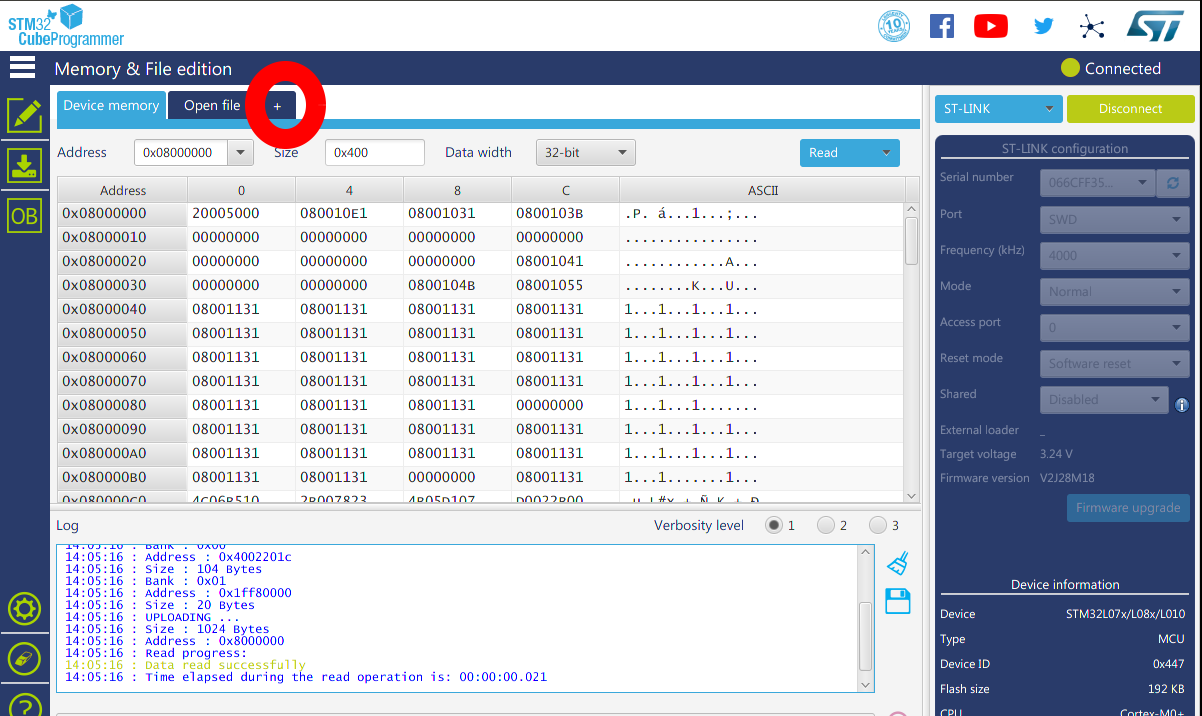
\includegraphics[keepaspectratio=true,scale=0.3]{st_cube_programmer_2.png}
\label{visina8}
\end{center}\end{figure}
    
    
  
   
\end{enumerate}

\end{document}
